%------------------------------------------------------------------------------
%Pevn� instalace
%------------------------------------------------------------------------------
\section{\texorpdfstring{Pevn� instalace}{Pevne instalace}}

  \begin{frame}
    \frametitle{Vliv harmonick�ch slo�ek na za��zen�}
  \end{frame}
%------------------------------------------------------------------------------	
  \begin{frame}
    \frametitle{Nap�ov� a proudov� nesymetrie 3f soustavy}
  \end{frame}
  
  \begin{frame}
    \frametitle{Symetriza�n� Steinmetz�v obvod}
  \end{frame}
  
  \begin{frame}
    \frametitle{Symetriza�n� obvod - P��klad}
    \begin{center}
		\begin{tabular}{c c}
			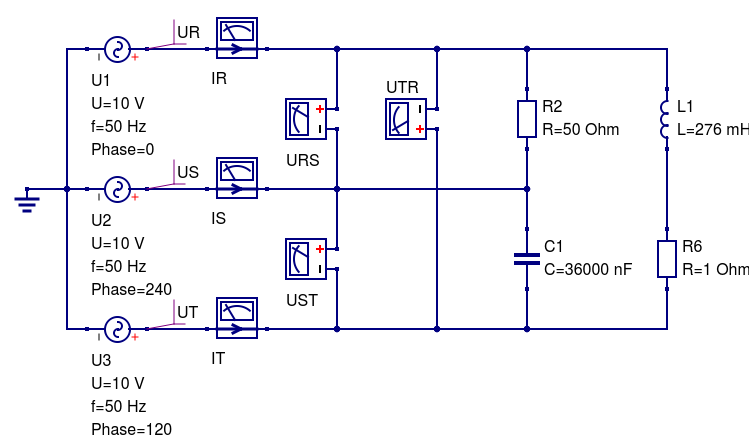
\includegraphics[width=0.45\linewidth]{sym_obv.png} &
			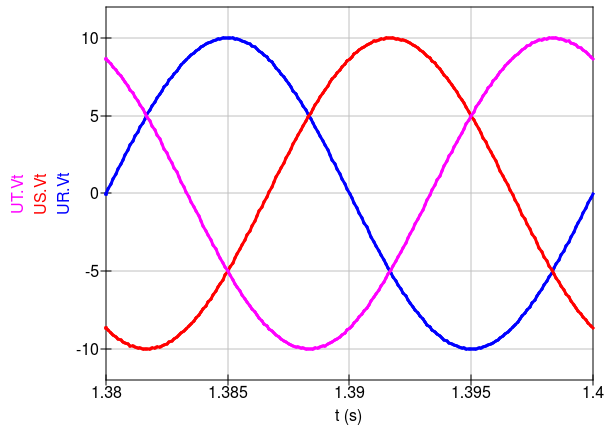
\includegraphics[width=0.46\linewidth]{sym_Vst.png}
		\end{tabular}
	\end{center}
  \end{frame}
  
  \begin{frame}
    \frametitle{Symetriza�n� obvod - P��klad}
    \begin{center}
		\begin{tabular}{c}
			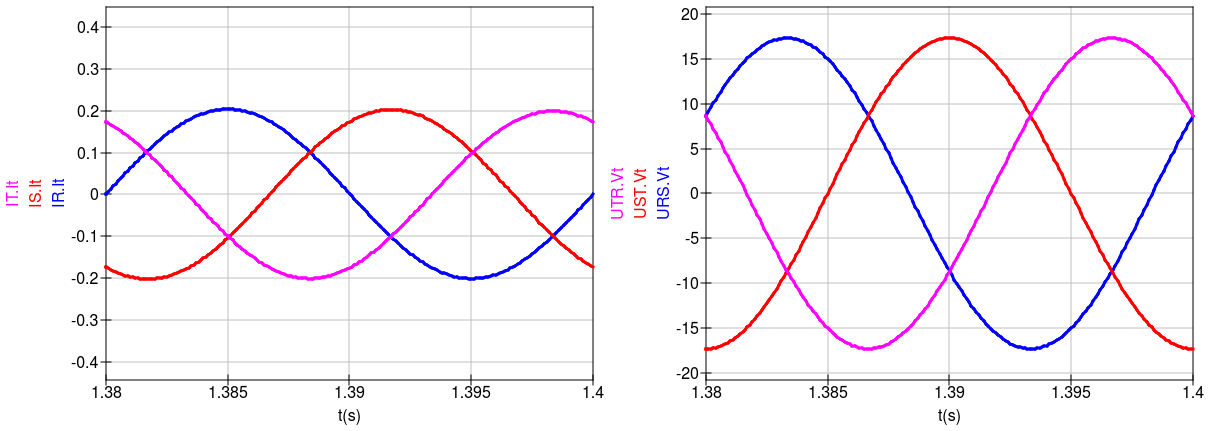
\includegraphics[width=0.9\linewidth]{sym_Vys.png}
		\end{tabular}
	\end{center}
  \end{frame}
	
  \begin{frame}
    \frametitle{P�ep�t�}
  \end{frame}
	
  \begin{frame}
    \frametitle{Zemn�n�}
  \end{frame}
	
  \begin{frame}
    \frametitle{Veden� kabel�}
  \end{frame}
	
  \begin{frame}
    \frametitle{P�ipojov�n� filtr�}
  \end{frame}
	
  \begin{frame}
    \frametitle{St�n�n�}
  \end{frame}